% Name: Projectile motion
% Description: A projectile's parabola from launch at angle θ, its initial velocity split into parts, the horizontal velocity at the top, the peak height, and the range.
% Tags: projectile, kinematics, parabola, velocity components

\usetikzlibrary{arrows.meta, angles, quotes}

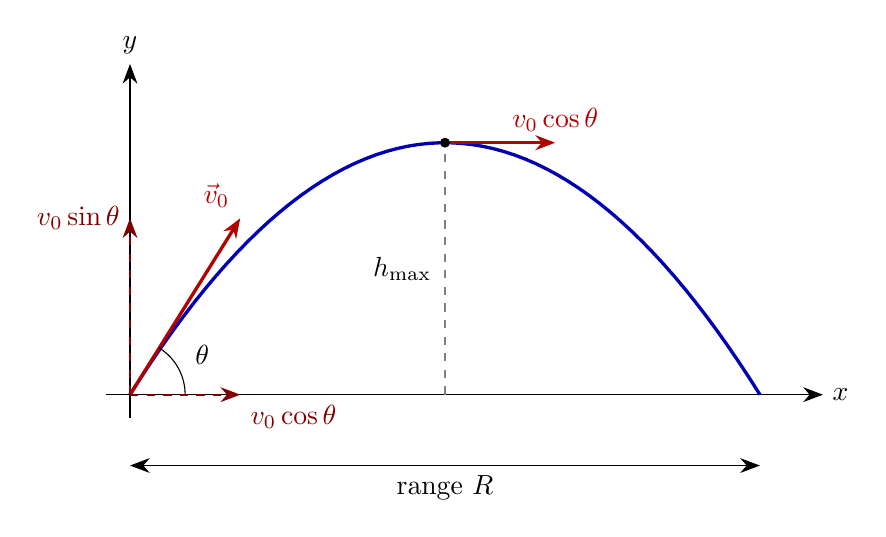
\begin{tikzpicture}[>={Stealth[length=2.5mm]}]
  \draw[->] (-0.3,0) -- (8.8,0) node[right] {$x$};
  \draw[->] (0,-0.3) -- (0,4.2) node[above] {$y$};
  \draw[very thick, blue!70!black, domain=0:8, samples=60] plot (\x, {0.2*\x*(8-\x)});
  \coordinate (O) at (0,0);
  \coordinate (X) at (1,0);
  \coordinate (V) at (1.4,2.24);
  \draw[->, very thick, red!70!black] (O) -- (V) node[above left] {$\vec{v}_0$};
  \draw[->, thick, dashed, red!50!black] (O) -- (1.4,0) node[below right] {$v_0\cos\theta$};
  \draw[->, thick, dashed, red!50!black] (O) -- (0,2.24) node[left] {$v_0\sin\theta$};
  \pic[draw, "$\theta$", angle eccentricity=1.5, angle radius=7mm] {angle = X--O--V};
  \draw[dashed, gray] (4,0) -- (4,3.2);
  \draw[->, very thick, red!70!black] (4,3.2) -- ++(1.4,0) node[above] {$v_0\cos\theta$};
  \fill (4,3.2) circle (1.8pt);
  \node[left] at (3.95,1.6) {$h_{\max}$};
  \draw[<->] (0,-0.9) -- node[below] {range $R$} (8,-0.9);
\end{tikzpicture}
